%!TEX root = p2p-private-cloud.tex

\section{Performance evaluation}%
\label{Performance}

To evaluate our protocol, we built a prototype of \name that implements the complete \name protocol in 5400 lines of Go code.
The users and their behavior (i.e. devices usage and file exchange decisions), on their part, are simulated by 1500 lines of Python.
Each device is a Docker container that ships the same \name code, and communicates with its peers via TCP connections.
To allow for realistic simulations (embodying more than 10 users), we distribute the experiments over 5 machines (one with an Intel Xeon E5-2660 CPU (32 cores) and 128GB of RAM, and four having an Intel Xeon E5420 CPU (8 cores) and 32GB of RAM), such that each \squad always resides on the same machine.
All peers are connected to the same Docker overlay network, and are thus reachable from any other device.

In the following, we first give precisions on the evaluation testbed and parameters in section~\ref{sub:evaluation_testbed}, before evaluating the PORs creation in section~\ref{sub:predictive_onion_routes_creation}, to conclude with an overall evaluation of the file transfer performance in section~\ref{sub:file_transfer}.

\subsection{Evaluation testbed} % (fold)
\label{sub:evaluation_testbed}

\subsubsection{Simulating user behavior} % (fold)
\label{ssub:simulating_user_behavior}

\newcommand\tuser{\ensuremath{t_{\text{user}}}}
\newcommand\ndevices{\ensuremath{n_{\text{devices}}}}

To evaluate \name, we take interest in users owning a variable amount of devices of different types, and frequently switching among them.
To the best of our knowledge, there exists no real-world dataset of the devices connection times of such a user.
On our testbed, each user's behavior is therefore simulated, according to the following rules:
\begin{itemize}
  \item The user owns a variable amount of devices. We consider the following device types: mobile (e.g. tablet, phone), portable (laptop), fixed (workstation, home computer) and server (such as a NAS, Raspberry Pi or rented appliance);
  \item The user always owns a phone;
	\item The user can travel between different locations;
	\item The user makes a different use of her devices depending on her location and device type: 
  her home computer will only be accessed at home, while her phone can be accessed everywhere (though she might tend to use it at home more than at work);
  \item The user's action are discretized: every action lasts the same amount of time \tuser.
\end{itemize}

Towards this goal, we model each user as a discrete time Hidden Markov Model (HMM) of order one. 
The hidden process $S=S_1, \dots, S_i, \dots$ represents the user's movements from one location from another, 
taken from the set of possible locations $\mathcal{S}$.
In our case, there are several independent observation processes (one per device), 
that form the observation sequence $O= O_1, \dots, O_i, \dots$.
$O_i[j]=1$ (resp. 0) means that the user's device $d_j$ was online (resp. offline) at time step $t_i$.

A HMM of order one is such that the current state $S_i$ (at time $t_i$) only depends on the previous one $S_{i-1}$ (at time $t_{i-1}$).
The observation at time $t_i$ ($O_i$) only depends on the current state $S_i$.

%locations, constituted of a set of $N$ potential locations (e.g. home, work or outside), $N$ being a user-defined parameter.


%We thus model each user with a Hidden Markov Model, as presented in section~\ref{sub:a_model_of_the_user_s_behavior}.
In detail, we applied the following rules to our models: 
\begin{itemize}
  \item There are three possible locations $\mathcal{S}=\left\{\text{Home}, \text{Outside}, \text{Work}\right\}$.
  Each user has transition probabilities from one place to another;
  one cannot go from work to home without transitionning outside and vice-versa;
  \item A user always has a phone, plus a random number of 2 to 9 devices which types are decided by a weighted random choice: each device has 30\% chances of being either mobile, portable, or fixed, and only 10\% probability of being a server;
  \item For each user, device, and location, the probability that a device be used at a location is picked at uniform random according to the following rules:
  \begin{itemize}
    \item \emph{Mobiles} can be accessed everywhere with a probability of 60 to 100\%;
    \item \emph{Portables} can be accessed everywhere with a probability of 20 to 80\%;
    \item \emph{Fixed} appliances can only be accessed from one single place (never outside) with a probability of 30 to 90\%;
    \item \emph{Servers} have a constant availability rate between 90 and 100\%.
  \end{itemize}
\end{itemize}

% we keep the different possible locations $\mathcal{L}$ to $N=3$ and the state transition matrix $A$ to a fixed value (cf figure~\ref{fig:hmm}).
% The number and types of devices per user, along with the matrix of emission probabilities $B$, is determined randomly according to the following rules.

% A user always has a phone, plus a random number of 2 to 9 devices whose type is decided by a weighted random choice: each device has 30\% chances of being either mobile, portable, or fixed, and only 10\% probability of being a server.
% $B_{*, d}$, the probability that device $d$ is used in each location, depends on $d$'s device type: 
% \begin{itemize}
% 	\item for each location, every mobile device $d_m$ has a random but high probability of being online: $\forall l \in \mathcal{L}, B_{l, d_m} \in [0.6, 1]$;
% 	\item a portable device $d_p$ has a much lower probability of being used: $\forall l \in \mathcal{L}, B_{l, d_p} \in [0.2, 0.8]$; 
% 	\item a fixed appliance $d_f$ has a non-zero probability of usage in only one location: $\exists l \in \mathcal{L}, B_{l, d_f} \in [0.4, 0.8] \text{ and } \forall l' \neq l, B_{l', d_f} = 0$;
% 	\item a server $d_s$ has a very high probability of working, whatever the user's location: $\exists p \in [0.9, 1], \forall l \in \mathcal{L}, B{l, d_s} = p$.
% \end{itemize} 

\begin{figure}[t]
\centering
\vspace{-1em}
\footnotesize
\centering
% $$A =
% \kbordermatrix{
%       & W   & O   & H   \cr
%     W & 0.6 & 0.4 & 0   \cr
%     O & 0.2 & 0.6 & 0.2 \cr
%     H & 0   & 0.4 & 0.6 \\[0.3em]
% }, \;
% B = 
% \kbordermatrix{
%       & W     & O   & H   \cr
%     p & 0.7 & 0.6 & 0.8 \cr
%     w & 0.7 & 0   & 0   \cr
%     h & 0   & 0   & 0.7 \cr
%     l & 0.2 & 0.4 & 0.6 \\[0.3em]
%}$$

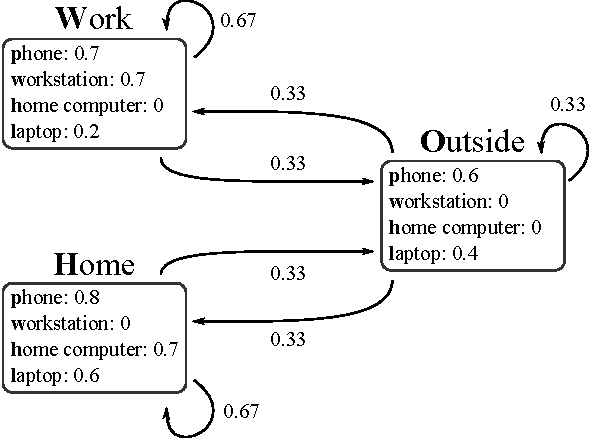
\includegraphics[width=0.65\columnwidth]{figures/hmm.pdf}
\vspace{2ex}
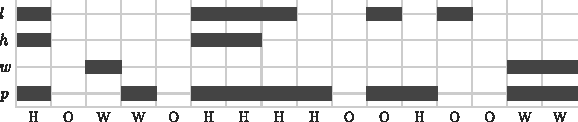
\includegraphics[width=0.9\columnwidth]{figures/sample_usage.pdf}

\caption{\label{fig:hmm} Example Hidden Markov Model (HMM) of a user's behavior. On top: visual representation of the model, with transition probabilities between locations and device usage probabilities at each location. On the bottom: Sample output from the HMM, with the initial of the location across time on the x-axis, the initial of each device on the y-axis, and their state across time (gray means online).}
\end{figure}

HMMs being generative probabilistic models, they allow the generation of observation sequences given the parameters of the model.
Figure~\ref{fig:hmm} shows a possible user's model along with a sample observation sequence $O$ generated from it.

Even though each user's behavior is discretized, they start at different times. 
This way, even though the time step \tuser is fixed, devices enter and leave the system at different points in the continuous time.


\subsubsection{Experimental parameters} % (fold)
\label{ssub:experimental_parameters}

All our experiments were conducted with 25 users participating in \name. 
The files exchanged are a collection of 12 real ones, ranging from 5KB to 640MB.

\paragraph*{Random Peer Sampling} It has three parameters: the period between two views exchange \trps, set to 400ms, the size of the exchanged views (6) and the size of the devices' view \rpsview, set to 30. 
Using a bigger view would result in more descriptors choice when crafting routes, but their descriptor would be more stale: descriptors in a view have a lifetime of $|\rpsview| * \trps$ seconds on average.

\paragraph*{Sprinkler} The \squad overlay has two parameters: the fanout of the gossip exchange when a device has new information to share, set to 3, and the initial length of the sequence $S$ (cf. section~\ref{ssec:device_availability}), set to 50.
The latter provides initial knowledge to \squad members: their peers addresses, among with an estimate of the user's prior behavior.

\paragraph*{PORs} We used a constant amount of 3 layers per routes (excluding the final, destination layer),
and a constant number of peers per layer $w_\layer$ of 16.
The latter heavily influences both the network overhead (the more, the bigger the headers), and the routes' availability (more peers means a better probability that at least one peer is online in a layer).
The default availability threshold $\theta$ is $10^-3$.

\paragraph*{File transfer} The main parameter here is the chunk size \chunksize, that was set to 512KB, which is considered, in BitTorrent, to be a good trade-off between network efficiency and number of chunks.
The other parameter, \tupload, was empirically set to 500ms.


\paragraph*{Users' behavior} Finally we set \tuser to 3s. 

\trps, \tupload and \tuser are correlated, but otherwise meaningless since \tuser is artificial. 
Their values were thus empirically chosen to balance efficiency, network traffic and the experiments' duration.

Finally, the experiments had a timeout of 15 minutes. 
We observed that downloads---however big---usually succeeded long before this time, or did not succeed whatever time was given to them.

\subsection{File transfer}
\label{sub:file_transfer}

\begin{figure}[t]
  \centering
  %\def\svgwidth{0.8\columnwidth}
  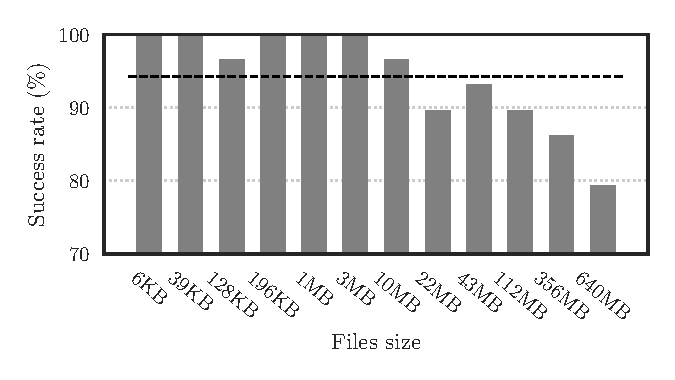
\includegraphics[width=0.8\columnwidth]{figures/completion_vs_size.pdf}

  \caption{\label{fig:completion_vs_size}
  Success rate of the file transfer ordered by size of file.}
\end{figure}


Using the previous parameters, we performed our experiment 30 times, yielding 360 file exchanges. Plots show the aggregation of the results from all experiments, which alleviates the high variability of the stochastic processes involved (most notably the devices' churn).

Overall, we saw 94\% of successful file transfer.

\begin{figure}[t]
  \centering
  %\def\svgwidth{0.8\columnwidth}
  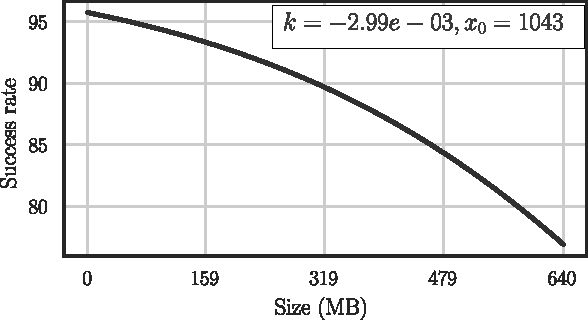
\includegraphics[width=0.8\columnwidth]{figures/logistic_many_0-001.pdf}

  \caption{\label{fig:logistic}
  Logistic regression of the success rate as a function of the file size using the default parameters.}
\end{figure}

Figure~\ref{fig:logistic} shows the logistic regression of the success rate as a function of the files' size. 
This regression is good candidate to describe binary stochastic processes as a function of a dependent variable,
and is often used in epidemics prediction, economics, and even marketing.
Simply put, given $X$ (in our case, the size of each transfered file) and $y$ (the outcome of the transfer: success or failure), 
the regressor estimates the coefficient $k$ and the mid-point $x_0$ of the logistic function defined as follows:

$$ f(x) = \frac{1}{1 + e^{-k \cdot x + x_0 }} $$

Because it sets the top (100\%) and bottom (0\%) values as asymptotes, 
logistic regression does not yield very optimistic success rates at the beginning,
but its midpoint $x_0$ tends to be very accurate even with a low quantity of training samples.
\commentAL{Yes indeed, very pessimistic, where is our 94\%!? I want to make a CDF also.}

In our case, $f(x)$ reads the probability that a file exchange fails given its size. 
The plot reads that files below 319MB have more than 90\% chances of being successfully exchanged.
The probability falls as the file gets bigger, such that a 1,O43MB has 50\% chances of successful transfer (see $x_0$).



\begin{figure}[t]
  \centering
  %\def\svgwidth{0.8\columnwidth}
  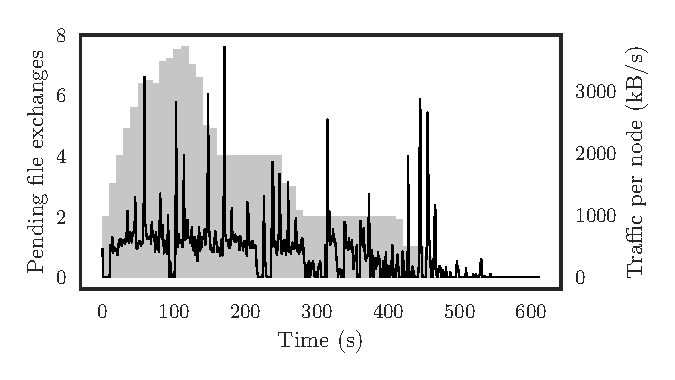
\includegraphics[width=\columnwidth]{figures/bw_and_pending_files.pdf}

  \caption{\label{fig:bw_and_pending_files}Traffic during one experiment.
  In gray: number of pending file exchanges; in black: mean outbound traffic (kB) per node per second.}
\end{figure}

\begin{figure}[t]
  \centering
  %\def\svgwidth{0.8\columnwidth}
  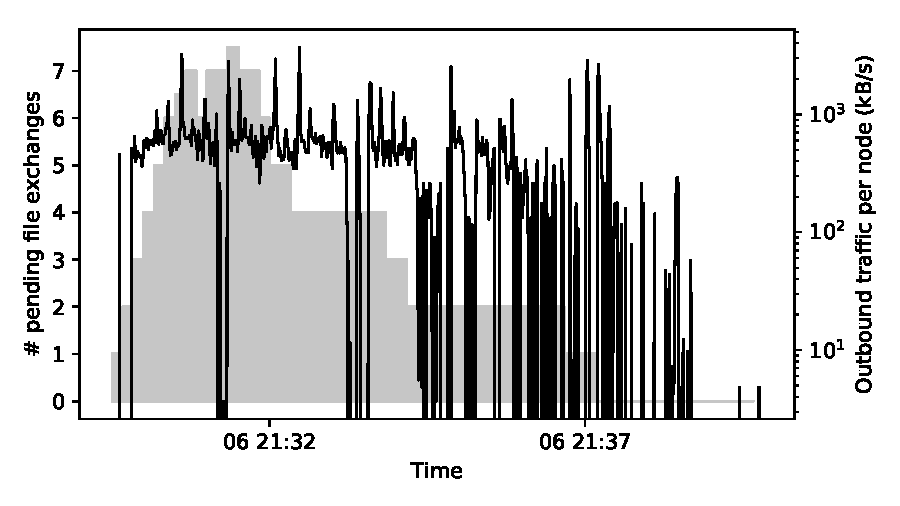
\includegraphics[width=\columnwidth]{figures/bw_and_pending_files_log.pdf}

  \caption{\label{fig:bw_and_pending_files_log}Traffic during one experiment.
  In gray: number of pending file exchanges; in black: mean outbound traffic (kB) per node per second.}
\end{figure}


% \subsection{Shortcomings} % (fold)
% \label{sub:shortcomings}

% There are several aspects in \name that can endanger its security or hinder its performance.
% First off, we study the RPS and its capacity to provide a random subset of the whole participants list.

% subsection shortcomings (end)


% In the following, we perform two types of experiments: 
% section~\ref{sub:predictive_onion_routes_creation} evaluates the establishment of PORs, while section~\ref{sub:file_transfer} handles file transfer.
% For that reason, they used different parameter sets.


% \paragraph*{PORs creation}
% Figure \ref{fig:success_rate_vs_t} come from the same data, with 10 experiments per set of settings.
% $\theta$, the threshold of the probability that all nodes fail at once, takes the following values: $[0.1, 0.01, 0.001, 0.0001]$.
% $L$, the number of layers constituting a route, takes the following values: $[3, 5, 7]$.
% The time since route establishment goes from 1 to 10 with  unit step.
% It is measured in time periods $T$, the interval at which users change the connection state of their devices.
% An experiment consisted in $L*5$ users, where we randomly picked pairs of users to compute 20 routes.
% Hence, each point on the top of figure~\ref{fig:success_rate_vs_t} is the average of 3000 layers size; 
% each point on the bottom is the availability rate over 200 routes.


% \paragraph*{File exchange}
% In section~\ref{sub:file_transfer}, we fix the routes' creation parameters: $\theta=10^-3$, $L=3$.
% The number of users is set to 20, and the number of file exchange per experiment to 10.
% We use a constant file chunk size of 512kB, a constant header size of 100kB, and a constant bandwidth per link of 128kB/s.


% \subsection{Predictive Onion Routes creation} % (fold)
% \label{sub:predictive_onion_routes_creation}

% We first measure the influence of the parameter $\theta$ on the number of nodes per layer on the top of figure~\ref{fig:success_rate_vs_t}, by displaying average and standard deviation of the number of nodes for $\theta=[10^{-4}, 10^{-3}, 10^{-2}, 10^{-1}]$ (the other experiment parameters are listed in section~\ref{ssub:experimental_parameters}).
% As we can see, the number of devices per layer logarithmically decreases as we relax the constraint on the layer's availability.
% The mean number of devices per layer lies between 2 and 6.
% Still, the number of nodes per layer is very variable: at $\theta=10^{-4}$, values range from 2 to 11, with a standard deviation of 1.44. 

% \begin{figure}[t]
% \centering
% 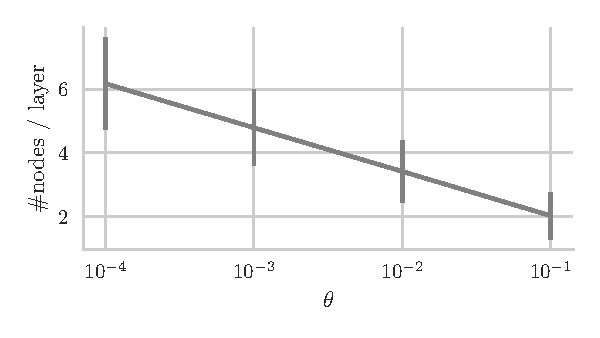
\includegraphics[width=0.7\columnwidth]{figures/nodes_per_layer_vs_theta.pdf}
% \vspace{1ex}
% 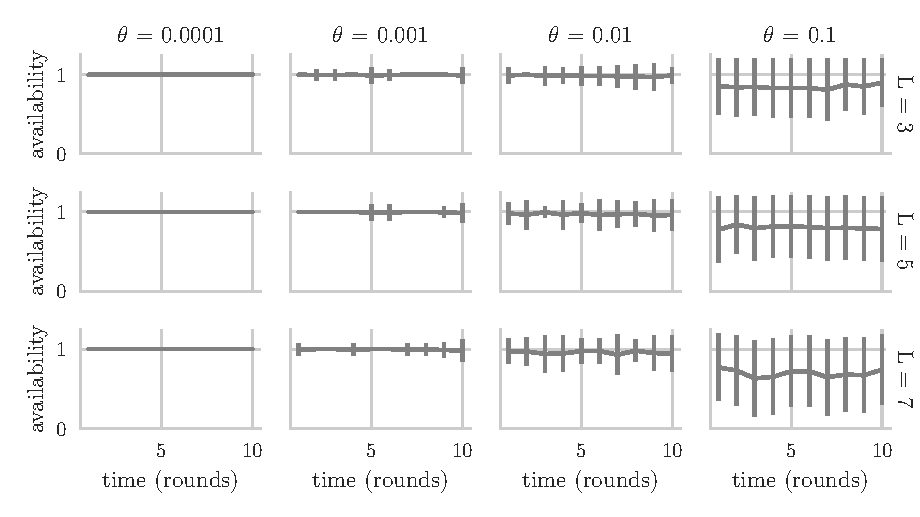
\includegraphics[width=0.9\columnwidth]{figures/success_rate_vs_t.pdf}
% \caption{\label{fig:success_rate_vs_t}On top: Number of nodes per layer of POR as a function of the parameter $\theta$ (the maximal probability that all nodes in a layer fail at once). The number of nodes logarithmically decreases as we relax the $\theta$ constraint. On bottom: Availability rate of routes as a function of the time since the route establishment, for several values of the parameters $\theta$ (the maximal probability that all nodes in a layer fail at once) and $L$ (the number of layers in the route).}
% \end{figure}

% We now study the influence of the parameters on the future availability of the routes in figure~\ref{fig:success_rate_vs_t}.
% We consider a route available if at least one node per layer is online at this time.
% The plots reads the mean availability of routes as a function of the time since the route's establishment, for every couple of parameters $(\theta, L)$.
% First of all, we observe that time has a negligible impact on the availability of routes. 
% This shows, as was stated in section~\ref{para:predicting future behavior}, that the prediction that devices make of behavior at $t+1$ is a good enough estimator for $t+i$.
% We also see that $\theta$ has a big impact on the mean availability and its variability.
% Still, $\theta\in\{10^-4, 10^-3\}$ allows highly available routes with an average availability of 100\% and 99.5\% respectively.
% Combined with the results from figure~\ref{fig:success_rate_vs_t}, it means that routes will need an average of 5-6 devices per layer to be highly available.
% Finally, increasing $L$ logically hinders the results when using low-availability layers.
% \\

% We showed that creating reliable onion routes using a backbone of unreliable nodes is feasible by using predictive algorithms.
% The counterpart is that messages header size grows with the number of layers and the number of devices per layer.

% Considering that most onion routing solutions use a statically defined message size to avoid information leakage, a bigger header means less space for the payload in each message. The more reliable the route, the bigger the number of messages per file. There is a trade-off between route reliability and network traffic.

% \subsection{File transfer time} % (fold)
% \label{sub:file_transfer}


% To assess the efficiency of \name, we did several file exchanges with fixed parameters and a random file size between 5MB and 500MB.
% By performing 20 experiments using the parameters described in \ref{ssub:experimental_parameters}, we obtained traces for 200 file exchanges.
% All files reached their destination successfully.

% \begin{figure}[t]
% \centering
% 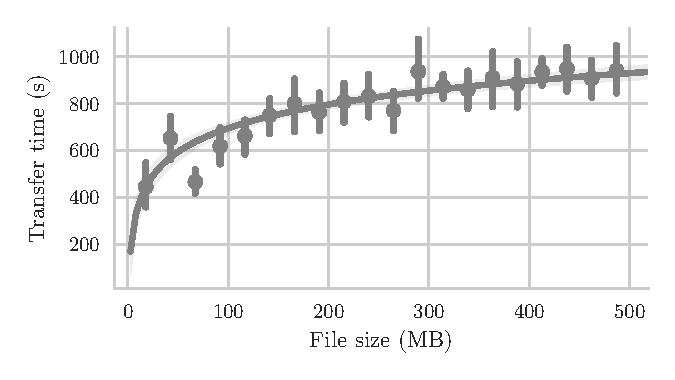
\includegraphics[width=0.7\columnwidth]{figures/transfer_time_vs_size.pdf}

% \caption{\label{fig:transfer_time_vs_size}Files' transfer time as a function of their size, along with a log-linear regression of the same data.}
% \end{figure}

% Figure~\ref{fig:transfer_time_vs_size} shows the results of this experiment: it plots the transfer time as a function of the file size. File size is binned into 20 bins, making the series of points representing the average transfer time per bin with standard deviation bars.
% We fitted a log-linear regression to this plot, displayed as a curve.
% It shows that transfer time increases less fast that the file size.

% Absolute time values are meaningless here: our system was evaluated on a single machine and on a single process. The code execution was not parallel, and only one device was executing at any point in time.

% Still, we investigated the message transmission. In this simulation, 145172 chunks were sent, and 141276 ACKs were received: 6.00\% of the chunks were lost in transit. A chunk took an average of 56s $\pm$ 36s to reach its destination, while ACKs to 48s $\pm$ 33s to do so. This is explained mostly by devices falling offline between the time they receive a message and the time they forward it.

% We now understand the log-linear curve and it's big initial slope: messages spend a long time in transit, but sending messages in parallel does not impact this time. Even small files thus need a lot of time to transfer, while bigger files do not suffer more than small files from the messages delay.
% \\

% Overall, we succeeded in creating a reliable and secure file transfer protocol over an underlying network of unreliable, low-end devices.
% Its performance could be enhanced by taking interest in bottlenecks in the messages transmission, i.e. scheduling messages in a similar predictive manner as we planned routes creation.




% subsection file_transfer (end)